% Master Thesis -- Final (Results) Presentation
% Style mirrors the proposal presentation (Beamer, Madrid theme, per-section TOC).
% Build: latexmk -pdf main.tex
%
% MTS requirements baked into this deck:
%   - Slide 1: (preliminary) thesis title + supervisor's name
%   - Research question stated by slide 3 at the latest
%   - One slide outlining the research design
%   - 20 minutes + 10 minutes discussion -> ~16 content slides + appendix
\documentclass[10pt]{beamer}

\usetheme{Madrid}

% Thesis colour scheme (see thesis_palette.R): indigo structure, teal alerts,
% so the deck matches the figures.
\definecolor{thesisindigo}{HTML}{3333AB}
\definecolor{thesisteal}{HTML}{008493}
\usecolortheme[named=thesisindigo]{structure}
\setbeamercolor{alerted text}{fg=thesisteal}

\usepackage[utf8]{inputenc}
\usepackage[T1]{fontenc}
\usepackage{amsmath,amssymb}
\usepackage{graphicx}
\usepackage{booktabs}
\usepackage{natbib}
\bibliographystyle{apalike}

% Notation (matches the thesis)
\newcommand{\CF}{\mathrm{CF}}
\newcommand{\GCF}{\mathrm{GCF}}
\newcommand{\FXGCF}{\mathrm{FXGCF}}
\newcommand{\rx}{\mathit{rx}}
\newcommand{\rxbar}{\overline{rx}}
\newcommand{\cyc}{c}                 % cycle
\newcommand{\cycbar}{\bar{c}}        % average cycle
\newcommand{\E}{\mathbb{E}}          % expectation
\DeclareMathOperator{\Corr}{Corr}

% Repeat the table of contents at every section start (as in the proposal)
\AtBeginSection[]{%
  \begin{frame}{Table of Contents}
    \tableofcontents[currentsection]
  \end{frame}}

\title[Expected Returns in Int'l Bond Markets]{Expected Returns in\\
  International Government Bond Markets}
\subtitle{Master Thesis -- Final Presentation}
\author[Jan Heissenberger]{Jan Heissenberger\\
  Supervised by Giorgia Simion, Ph.D.}
\date{June 2026} % TODO: set the exact presentation date once the schedule is announced

\begin{document}

% --------------------------------------------------------------------------
% Slide 1: title, supervisor (MTS requirement)
\begin{frame}
  \titlepage
\end{frame}

% Slide 2: TOC
\begin{frame}{Table of Contents}
  \tableofcontents
\end{frame}

% --------------------------------------------------------------------------
\section{Research Question}

% Slide 3: research question (MTS requirement: by slide 3 at the latest)
\begin{frame}{Research Question}
  \begin{block}{Main Question}
    Does the \citet{cieslak2015} cycle factor (CF) apply to international
    bonds?\\
    {\small\color{gray} If their propositions hold, the mechanism found in the
    US market should be fundamental to bond markets in other developed
    countries.}
  \end{block}
  \textbf{Subquestions}
  \begin{enumerate}
    \item What is the role of the local CF in comparison to a GDP-weighted
      global CF ($\GCF$)?
    \item Does a global CF subsume the predictive power of a local CF?
    \item Does currency risk break the predictability for a USD investor, and
      does an FX-adjusted global factor ($\FXGCF$) restore it?
  \end{enumerate}
\end{frame}

\begin{frame}{Recap: The Cycle-Factor Framework}
  Yields decompose into slow-moving \emph{trend inflation} and transitory
  \emph{cycles} \citep{cieslak2015}:
  \begin{equation*}
    y^{(n)}_{i,t} \;=\; \alpha_{i,n} \;+\; \beta_{i,n}\,\pi^{e}_{i,t}
      \;+\; \underbrace{c^{(n)}_{i,t}}_{\text{cycle}}
  \end{equation*}
  The cycles forecast one-year-ahead, duration-standardised,
  maturity-averaged excess returns $\rxbar_{i,t+12}$.
  \vfill
  \textbf{Factor hierarchy}
  \begin{enumerate}
    \item \textbf{Local} $\CF_{i,t}$: fitted return forecast from
      $c^{(1)}_{i,t}$ and the average cycle $\bar c_{i,t}$
    \item \textbf{Global} $\GCF_{t} = \sum_{i} w_{i,t}\,\CF_{i,t}$:
      GDP-weighted shared risk \citep{dahlquist2013}
    \item \textbf{FX-adjusted global} $\FXGCF_{t}$: built on the GDP-weighted
      average \emph{USD} return for an unhedged US investor
  \end{enumerate}
\end{frame}

% --------------------------------------------------------------------------
\section{Research Design \& Data}

% MTS requirement: one slide outlining the research design
\begin{frame}{Research Design}
  \textbf{Sample:} G10 markets, monthly zero-coupon yields, core CPI, FX spot
  rates, nominal GDP; 1994--2026.
  \vfill
  \textbf{Three empirical phases} (in-sample, Newey--West HAC inference)
  \begin{itemize}
    \item[\textbf{I}] Local predictability:
      $\rxbar_{i,t+12}=\alpha_i+\beta_i\,\CF_{i,t}+\varepsilon$ per country
    \item[\textbf{II}] Integration horse race:
      $\rxbar_{i,t+12}=\alpha_i+\beta_i\,\CF^{\perp}_{i,t}
        +\gamma_i\,\GCF_{t}+\varepsilon$
    \item[\textbf{III}] USD investor:
      $rx^{\mathrm{USD}}_{i,t+12}$ on $\GCF_{t}$ vs.\ $\FXGCF_{t}$
  \end{itemize}
  \vfill
  \textbf{Validation \& stress tests}
  \begin{itemize}
    \item Replication of \citet{cieslak2015} and \citet{dahlquist2013} on US /
      international data before any extension
    \item $R^{2}$ benchmarked against an expectations-hypothesis Monte Carlo
    \item Fully-recursive out-of-sample evaluation
      \citep[Campbell--Thompson $R^{2}_{\mathrm{oos}}$;][]{campbellthompson2008}
    \item Robustness: crisis subsamples, rolling windows, CF vs.\ CP factor,
      core vs.\ headline inflation
  \end{itemize}
\end{frame}

\begin{frame}{Data \& Validation}
  \begin{itemize}
    \item \textbf{Universe:} G10 (BE, CA, FR, DE, IT, JP, NL, SE, CH, UK, US)
    \item \textbf{Yields:} zero-coupon curves, maturities 1, 2, 4, 5, 9, 10
      years (Bloomberg); \textbf{inflation:} core CPI (LSEG); \textbf{FX} spot
      vs.\ USD; \textbf{GDP:} nominal (LSEG)
    \item \textbf{Frequency / span:} monthly, 1994--2026; returns are
      one-year-ahead, duration-standardised, maturity-averaged
  \end{itemize}
  \vfill
  \begin{block}{Replication as validation}
    The estimation engine reproduces the published US evidence: the
    return-forecasting factor correlates $0.69$ with the average cycle
    (vs.\ $0.61$ reported by \citealp{cieslak2015}) and recovers the published
    sign pattern, before the framework is taken international.
  \end{block}
\end{frame}

% --------------------------------------------------------------------------
\section{Results}

\begin{frame}{Phase I --- The Local Cycle Factor Works Across the G10}
  \begin{columns}[T]
    \begin{column}{0.52\textwidth}
      \begin{itemize}
        \item Sign pattern of \citet{cieslak2015} ($\gamma_{1}<0$ on the
          1y cycle, $\gamma_{2}>0$ on the average cycle) in \textbf{all 11
          markets}
        \item Joint Wald rejects no-predictability at 1\% in 9 countries,
          at 5\% in 10 (exception: Switzerland, $p=0.20$)
        \item Pooled panel: $t=-10.7$ and $t=15.5$
        \item In-sample $R^{2}$: 7\% (CH) to 34\% (NL), \textbf{average
          25\%}; US 33\% --- matching the original study
        \item Far above the EH Monte-Carlo 95th percentile; holds at every
          maturity ($n=2,5,10$)
      \end{itemize}
    \end{column}
    \begin{column}{0.46\textwidth}
      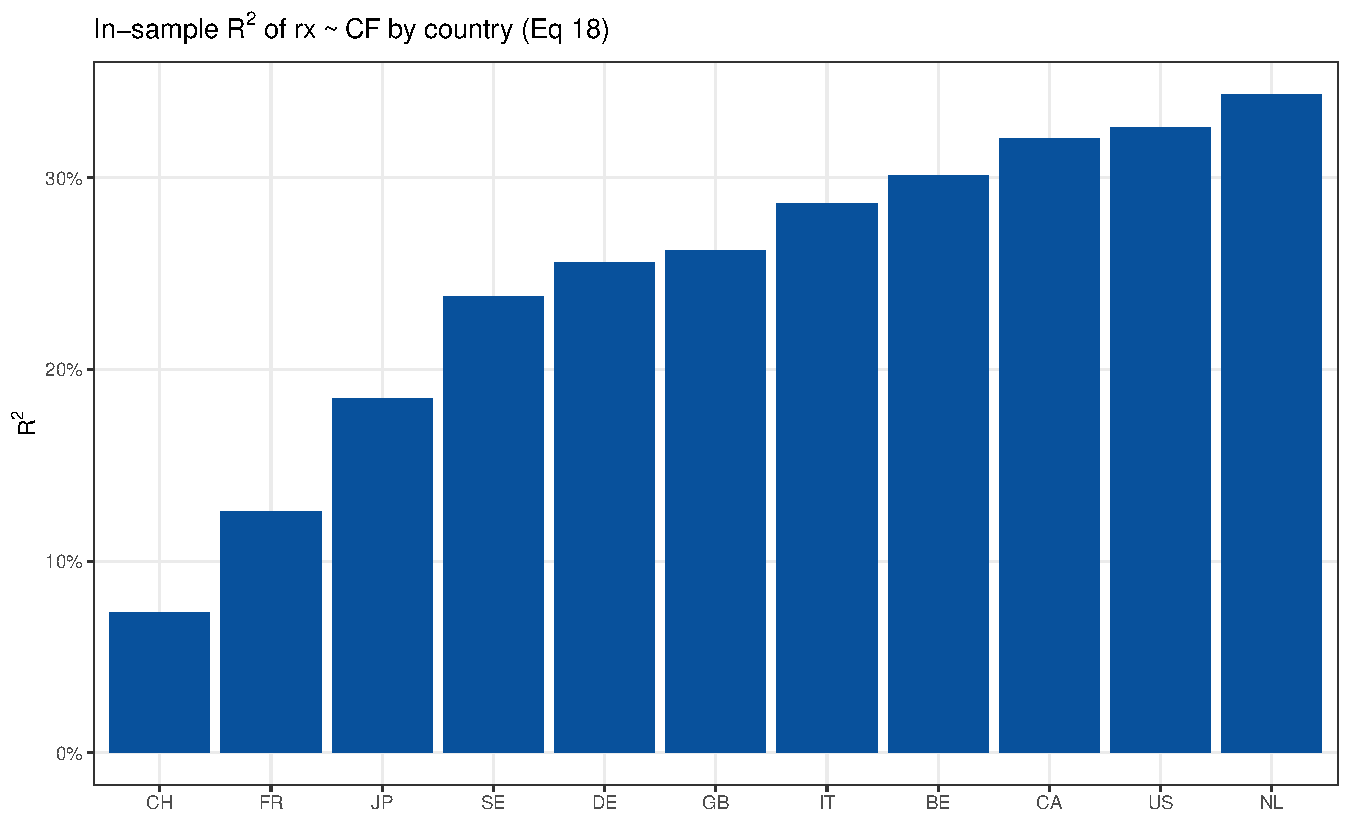
\includegraphics[width=\linewidth]{figures/mr_f1_r2_phase1.pdf}
      {\scriptsize In-sample $R^{2}$ of $\rxbar_{i,t+12}\sim\CF_{i,t}$ by
        country.}
    \end{column}
  \end{columns}
\end{frame}

\begin{frame}{Phase II --- One Global Factor Summarises Eleven Local Ones}
  \centering
  
\includegraphics[width=0.62\linewidth]{figures/s5_gcf.pdf}
  \begin{itemize}
    \item $\GCF_{t}$ (GDP-weighted) tracks the centre of mass of the eleven
      local factors
    \item On its own it matches the local factors' explanatory power:
      average $R^{2}$ of \textbf{25\% vs.\ 25\%}
  \end{itemize}
\end{frame}

\begin{frame}{Phase II --- The Global Factor Largely Subsumes the Local}
  \begin{columns}[T]
    \begin{column}{0.5\textwidth}
      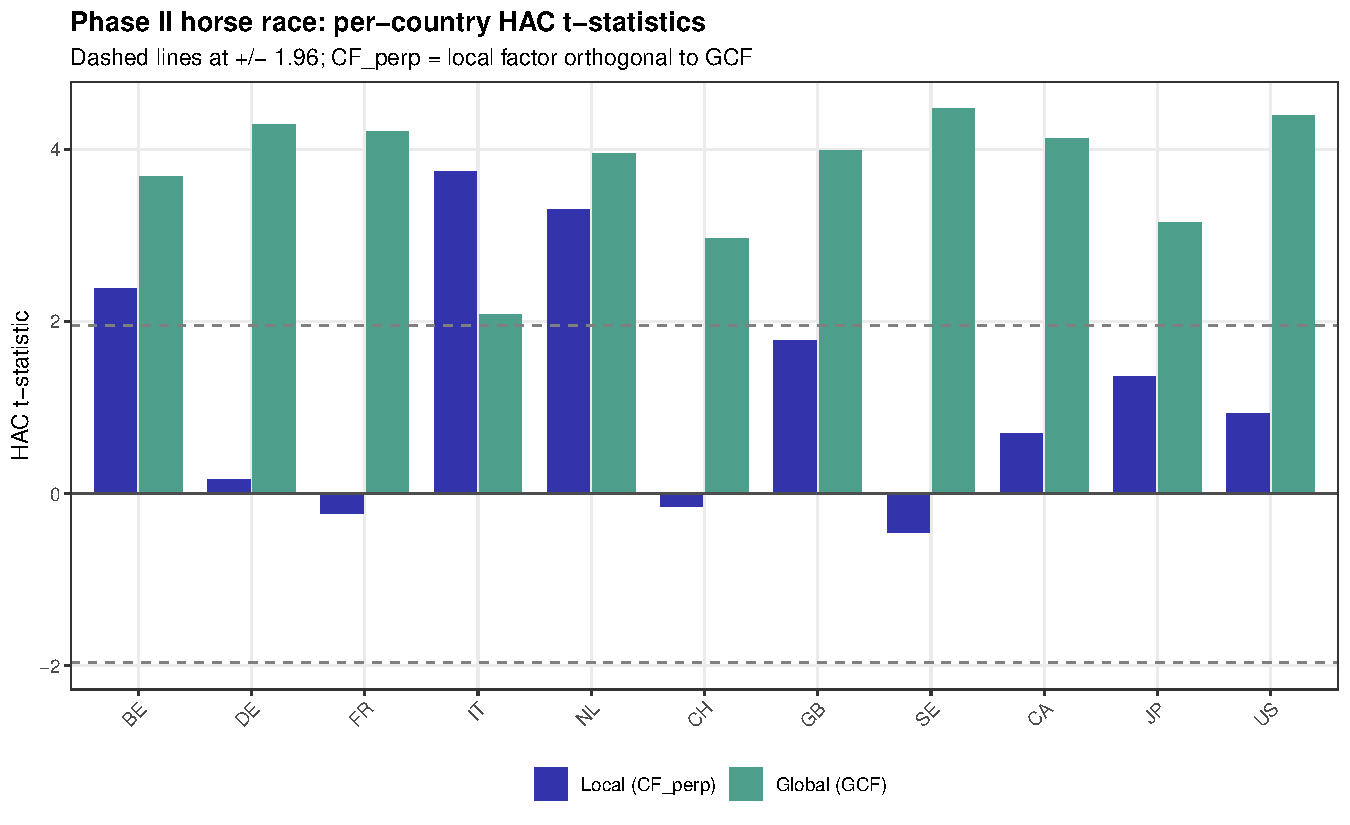
\includegraphics[width=\linewidth]{figures/mr_f2_hr_tstats.pdf}
      {\scriptsize HAC $t$-statistics in the horse race
        $\rxbar\sim\CF^{\perp}+\GCF$; dashed lines $\pm1.96$.}
    \end{column}
    \begin{column}{0.48\textwidth}
      \begin{itemize}
        \item $\GCF$ significant in \textbf{every} market
          ($t$ between 2.1 and 4.5)
        \item Orthogonalised local factor survives in only
          \textbf{3 of 11} markets: Italy ($t=3.7$), Netherlands ($t=3.3$),
          Belgium ($t=2.4$)
        \item Where subsumed, adding $\CF^{\perp}$ lifts $R^{2}$ only
          trivially (DE: $28.4\%\to28.4\%$)
        \item Strong --- but incomplete --- integration of bond risk premia
          \citep{dahlquist2013}; euro-area exceptions plausibly reflect
          sovereign-spread dynamics
      \end{itemize}
    \end{column}
  \end{columns}
\end{frame}

\begin{frame}{Phase III --- Currency Risk Breaks It for the USD Investor}
  \begin{columns}[T]
    \begin{column}{0.5\textwidth}
      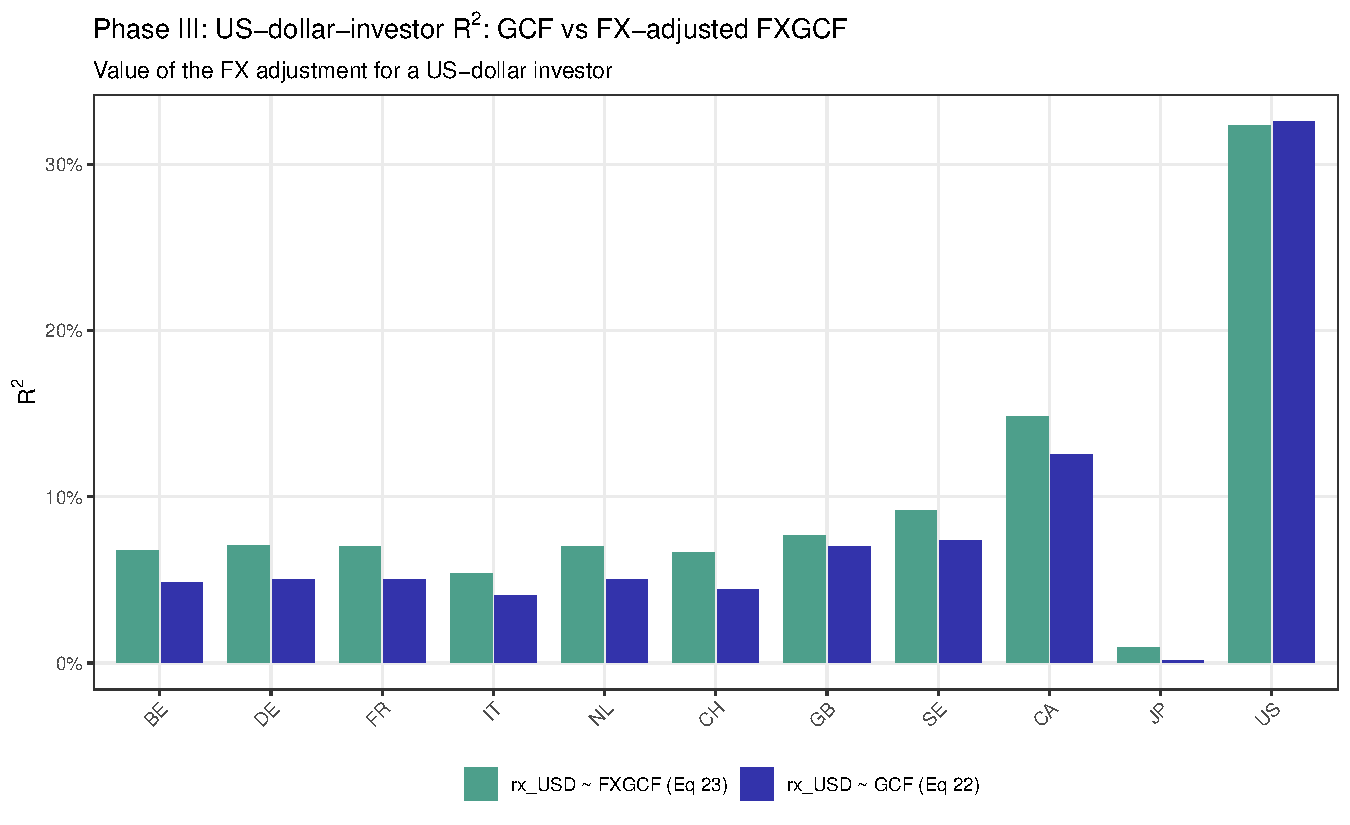
\includegraphics[width=\linewidth]{figures/mr_f3_usd_r2.pdf}
      {\scriptsize USD-investor in-sample $R^{2}$: $\GCF$ vs.\ $\FXGCF$.}
    \end{column}
    \begin{column}{0.48\textwidth}
      \begin{itemize}
        \item Average $R^{2}$ collapses from \textbf{25\% (local currency) to
          8\% (USD returns)}
        \item Significance lost across the euro area, Switzerland, Japan;
          survives in US (33\%), Canada ($t=2.9$), marginally SE and UK
        \item One-year FX volatility swamps the cyclical bond signal
      \end{itemize}
    \end{column}
  \end{columns}
\end{frame}

\begin{frame}{Phase III --- The FX Adjustment Helps, but Modestly}
  \begin{columns}[T]
    \begin{column}{0.5\textwidth}
      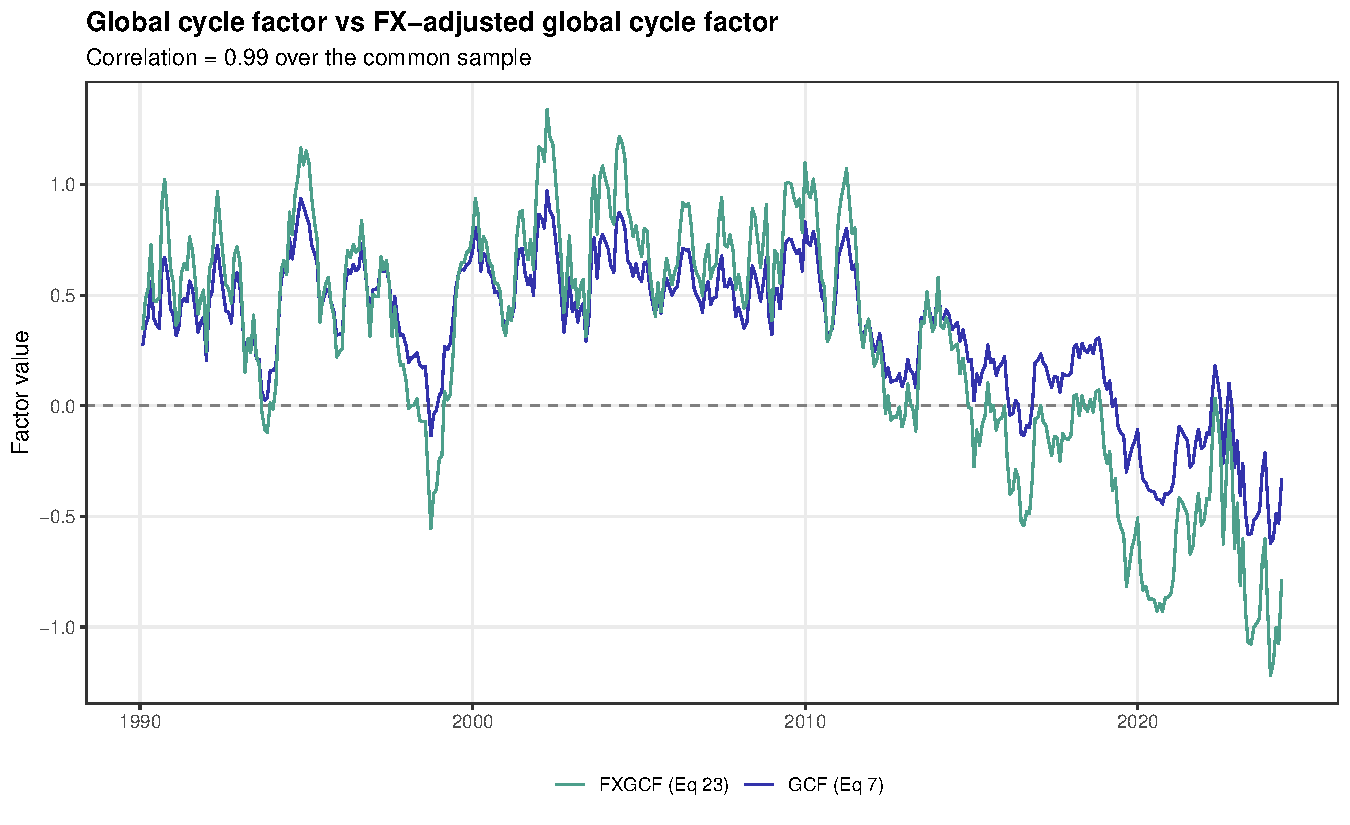
\includegraphics[width=\linewidth]{figures/mr_f4_gcf_fxgcf.pdf}
      {\scriptsize $\GCF_{t}$ and $\FXGCF_{t}$: correlation $0.99$.}
    \end{column}
    \begin{column}{0.48\textwidth}
      \begin{itemize}
        \item $\FXGCF$ raises the USD-investor $R^{2}$ in \textbf{10 of 11}
          markets and the $t$-statistic in every foreign market
        \item Average $R^{2}$: $8\%\to10\%$; direction uniform, magnitude
          small
        \item Reason: $\FXGCF$ correlates \textbf{0.99} with $\GCF$ in this
          sample --- vs.\ $\approx0.50$ in \citet{dahlquist2013} --- a
          substantive finding in its own right
      \end{itemize}
    \end{column}
  \end{columns}
\end{frame}

\begin{frame}{Out of Sample --- Only the Global Factor Survives Real Time}
  \begin{columns}[T]
    \begin{column}{0.5\textwidth}
      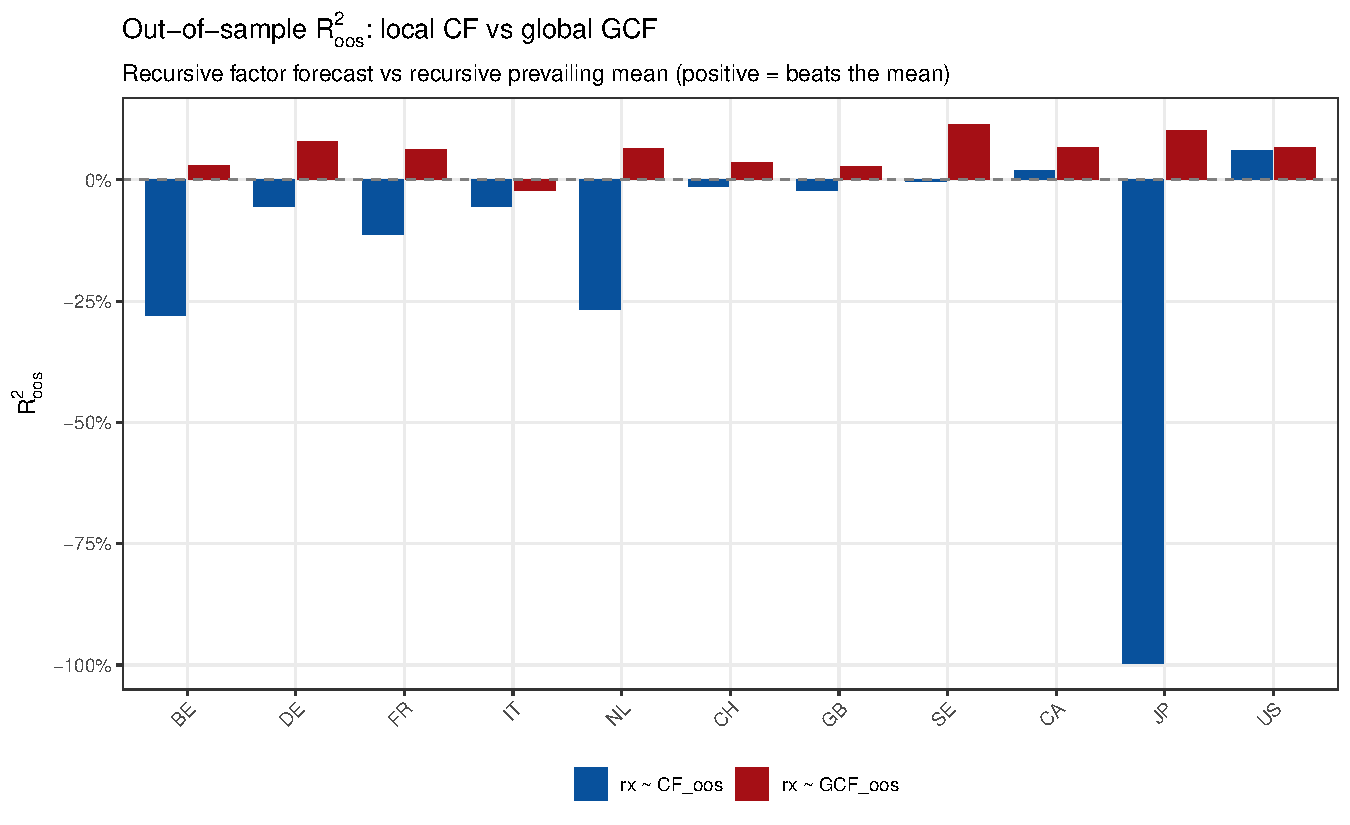
\includegraphics[width=\linewidth]{figures/mr_f5_oos_r2.pdf}
      {\scriptsize Campbell--Thompson $R^{2}_{\mathrm{oos}}$ vs.\ the
        recursive prevailing mean, by country.}
    \end{column}
    \begin{column}{0.48\textwidth}
      Fully-recursive: decomposition, regressions and aggregation rebuilt at
      each date from past data only.
      \begin{itemize}
        \item \textbf{Local CF:} pooled $R^{2}_{\mathrm{oos}}=-0.08$;
          beats the mean in only 2 of 11 markets --- the in-sample fit is
          largely generated-regressor over-fit
        \item \textbf{Global $\GCF$:} pooled $\mathbf{+0.05}$, positive in
          \textbf{10 of 11} markets --- the strongest integration evidence in
          the thesis
        \item \textbf{USD investor:} $\GCF$ at $-0.07$; $\FXGCF$ turns it
          marginally positive ($+0.002$, 9 of 11 markets), but the edge is
          thin and fragile
      \end{itemize}
    \end{column}
  \end{columns}
\end{frame}

\begin{frame}{Economic Value --- Timing a Global Bond Portfolio}
  \begin{columns}[T]
    \begin{column}{0.5\textwidth}
      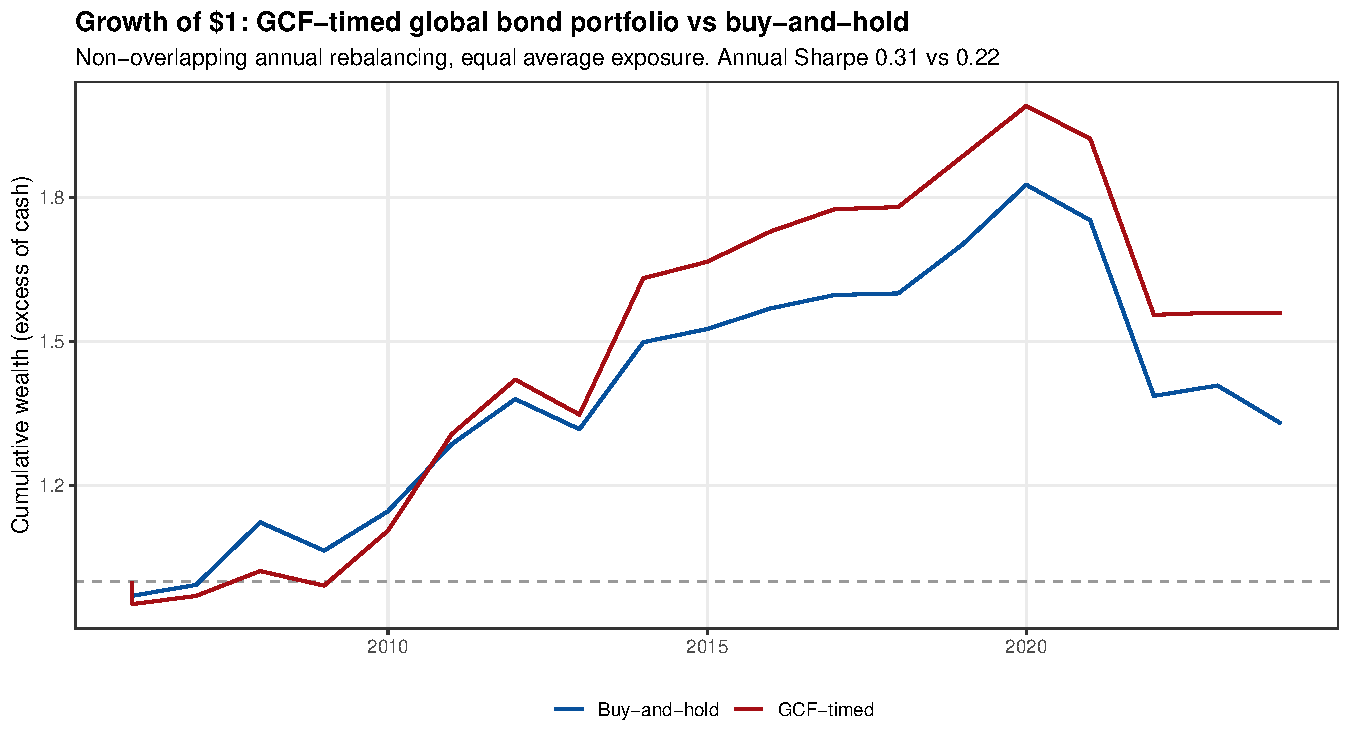
\includegraphics[width=\linewidth]{figures/strat_f1_cumret.pdf}
      {\scriptsize Out-of-sample cumulative returns, 2005--2024.}
    \end{column}
    \begin{column}{0.48\textwidth}
      Mean--variance timing of a GDP-weighted 10y global bond portfolio on the
      recursive $\GCF$ forecast (currency-hedged investor):
      \begin{itemize}
        \item Portfolio-level $R^{2}_{\mathrm{oos}}=0.125$
        \item Sharpe ratio: \textbf{0.31 (passive) $\to$ 0.38}; 0.34 for
          mean-timing
        \item Certainty-equivalent gain ($\gamma=5$): \textbf{+0.51\%/yr} over
          buy-and-hold, +0.30\% over mean-timing
        \item Modest in magnitude, but real-time implementable end to end
      \end{itemize}
    \end{column}
  \end{columns}
\end{frame}

\begin{frame}{Robustness --- What Survives, What Is Fragile}
  \textbf{Survives every test}
  \begin{itemize}
    \item The GDP-weighted global cycle factor: in-sample and out-of-sample,
      across subsamples (except the GFC itself), with core inflation, and
      against the Cochrane--Piazzesi forward-rate factor
    \item Construction choices (EWMA decay $v$, window $M$, maturity menu, GDP
      weights) move results little
  \end{itemize}
  \vfill
  \textbf{Fragile}
  \begin{itemize}
    \item Local-factor predictability does not survive real-time evaluation
    \item USD-investor predictability is regime-dependent (concentrated
      pre-2008)
    \item The $\FXGCF$ edge is concentrated post-crisis and does not survive a
      rolling estimation window
  \end{itemize}
\end{frame}

% --------------------------------------------------------------------------
\section{Conclusion}

\begin{frame}{Conclusion}
  \begin{block}{Does the \citet{cieslak2015} cycle factor apply to
      international bonds? --- Yes.}
    Correct sign structure in all 11 G10 markets, average in-sample
    $R^{2}=25\%$, at every maturity.
  \end{block}
  \begin{enumerate}
    \item \textbf{Local vs.\ global:} one GDP-weighted global factor matches
      eleven national factors (25\% vs.\ 25\%) and is significant everywhere.
    \item \textbf{Subsumption:} the global factor drives out the local one in
      8 of 11 markets; predictability is overwhelmingly global --- and only
      the global factor predicts \emph{out of sample}.
    \item \textbf{USD investor:} currency risk erodes $\sim$2/3 of the
      predictive power; the novel $\FXGCF$ restores it in direction but only
      partially --- it is near-collinear (0.99) with $\GCF$ in this sample.
  \end{enumerate}
  \vfill
  \textbf{Contribution:} a unified global cycle factor for the G10, its
  FX-adjusted variant, and real-time evidence (incl.\ economic value) that
  international bond-return predictability is a global, macro-anchored
  phenomenon.
\end{frame}

\begin{frame}{Bibliography}
  \small
  \bibliography{references}
\end{frame}

% --------------------------------------------------------------------------
\appendix
\section{Appendix}

\begin{frame}{Appendix: Phase I --- Full Country Table}
  \centering
  % mr_t1_phase1 — Phase I: local cycle-factor predictability across the G10.
% Native-LaTeX version for the deck; numbers match thesis/tables/mr_t1_phase1.tex
% (generated by main_results.R). Replaces the former PDF screenshot.
\resizebox{\linewidth}{!}{%
\begin{tabular}{l cc cc c c r}
  \toprule
  & \multicolumn{2}{c}{$\cyc^{(1)}_{i,t}$} & \multicolumn{2}{c}{$\cycbar_{i,t}$} & & & \\
  \cmidrule(lr){2-3}\cmidrule(lr){4-5}
  Country & $\hat{\gamma}_{1}$ & $t$ & $\hat{\gamma}_{2}$ & $t$ & $R^{2}$ & Wald $p$ & $N$ \\
  \midrule
  Belgium        & $-0.42$ & $(-3.42)$  & $0.56$ & $(4.61)$  & $0.301$ & $0.000$ & $353$ \\
  Germany        & $-0.34$ & $(-3.27)$  & $0.47$ & $(4.82)$  & $0.256$ & $0.000$ & $353$ \\
  France         & $-0.39$ & $(-4.02)$  & $0.51$ & $(4.26)$  & $0.126$ & $0.000$ & $353$ \\
  Italy          & $-0.26$ & $(-1.46)$  & $0.59$ & $(3.19)$  & $0.287$ & $0.000$ & $353$ \\
  Netherlands    & $-0.36$ & $(-3.18)$  & $0.56$ & $(5.46)$  & $0.344$ & $0.000$ & $353$ \\
  Switzerland    & $-0.11$ & $(-1.17)$  & $0.26$ & $(1.77)$  & $0.073$ & $0.201$ & $353$ \\
  United Kingdom & $-0.41$ & $(-4.36)$  & $0.54$ & $(4.54)$  & $0.262$ & $0.000$ & $353$ \\
  Sweden         & $-0.26$ & $(-1.91)$  & $0.43$ & $(3.33)$  & $0.238$ & $0.001$ & $353$ \\
  Canada         & $-0.22$ & $(-2.37)$  & $0.41$ & $(4.36)$  & $0.320$ & $0.000$ & $353$ \\
  Japan          & $-0.30$ & $(-1.48)$  & $0.46$ & $(2.12)$  & $0.185$ & $0.023$ & $367$ \\
  United States  & $-0.40$ & $(-3.21)$  & $0.79$ & $(4.30)$  & $0.326$ & $0.000$ & $412$ \\
  \midrule
  G10 panel      & $-0.33$ & $(-10.72)$ & $0.51$ & $(15.45)$ & $0.253$ & $0.000$ & $3956$ \\
  \bottomrule
\end{tabular}}\\[0.8ex]
{\scriptsize\begin{minipage}{0.92\linewidth}
  Predictive regression
  $\rxbar_{i,t+12}=\gamma_{0}+\gamma_{1}\cyc^{(1)}_{i,t}+\gamma_{2}\cycbar_{i,t}
  +\varepsilon$; the local factor $\CF_{i,t}$ is its fitted value.
  Newey--West HAC $t$-statistics (12-month overlap) in parentheses; Wald $p$ is
  the joint test that both cycle slopes are zero. $R^{2}$ is in-sample; the G10
  panel pools all countries with country fixed effects.
\end{minipage}}

\end{frame}

\begin{frame}{Appendix: Phase II --- Horse-Race Table}
  \centering
  % mr_t2_phase2 — Phase II: global vs local cycle factor (horse race).
% Native-LaTeX version for the deck, numbers match thesis/tables/mr_t2_phase2.tex
% (generated by main_results.R). Replaces the former PDF screenshot.
\resizebox{\linewidth}{!}{%
\begin{tabular}{l ccc cc cc}
  \toprule
  & \multicolumn{3}{c}{$R^{2}$} & \multicolumn{2}{c}{HAC $t$} & & \\
  \cmidrule(lr){2-4}\cmidrule(lr){5-6}
  Country & $\CF$ & $\GCF$ & Joint & $\CF^{\perp}$ & $\GCF$ & Wald $p$ & $p$ (BH) \\
  \midrule
  Belgium        & $0.301$ & $0.209$ & $0.301$ & $2.38$  & $3.69$ & $0.000$ & $0.000$ \\
  Germany        & $0.256$ & $0.284$ & $0.284$ & $0.16$  & $4.30$ & $0.000$ & $0.000$ \\
  France         & $0.126$ & $0.260$ & $0.261$ & $-0.23$ & $4.21$ & $0.000$ & $0.000$ \\
  Italy          & $0.287$ & $0.074$ & $0.315$ & $3.75$  & $2.08$ & $0.000$ & $0.000$ \\
  Netherlands    & $0.344$ & $0.263$ & $0.350$ & $3.30$  & $3.96$ & $0.000$ & $0.000$ \\
  Switzerland    & $0.073$ & $0.194$ & $0.194$ & $-0.15$ & $2.97$ & $0.012$ & $0.012$ \\
  United Kingdom & $0.262$ & $0.261$ & $0.286$ & $1.78$  & $4.00$ & $0.000$ & $0.000$ \\
  Sweden         & $0.238$ & $0.291$ & $0.293$ & $-0.45$ & $4.48$ & $0.000$ & $0.000$ \\
  Canada         & $0.320$ & $0.352$ & $0.358$ & $0.70$  & $4.14$ & $0.000$ & $0.000$ \\
  Japan          & $0.185$ & $0.202$ & $0.224$ & $1.36$  & $3.15$ & $0.007$ & $0.007$ \\
  United States  & $0.326$ & $0.326$ & $0.333$ & $0.93$  & $4.39$ & $0.000$ & $0.000$ \\
  \bottomrule
\end{tabular}}\\[0.8ex]
{\scriptsize\begin{minipage}{0.92\linewidth}
  Horse race
  $\rxbar_{i,t+12}=\alpha_i+\beta_i\,\CF^{\perp}_{i,t}+\gamma_i\,\GCF_{t}
  +\varepsilon$, where $\CF^{\perp}_{i,t}$ is the local factor orthogonalised to
  $\GCF_{t}$ \citep{dahlquist2013}. The $\CF$/$\GCF$ columns under $R^{2}$ are the
  single-factor fits, and Joint is the horse-race fit. HAC $t$ are Newey--West
  $t$-statistics on the two slopes. $p$ (BH) is the Benjamini--Hochberg
  FDR-adjusted Wald $p$. A significant $\GCF$ with an insignificant $\CF^{\perp}$
  means the global factor subsumes the local one.
\end{minipage}}

\end{frame}

\begin{frame}{Appendix: Phase II --- $R^{2}$ Ladder}
  \centering
  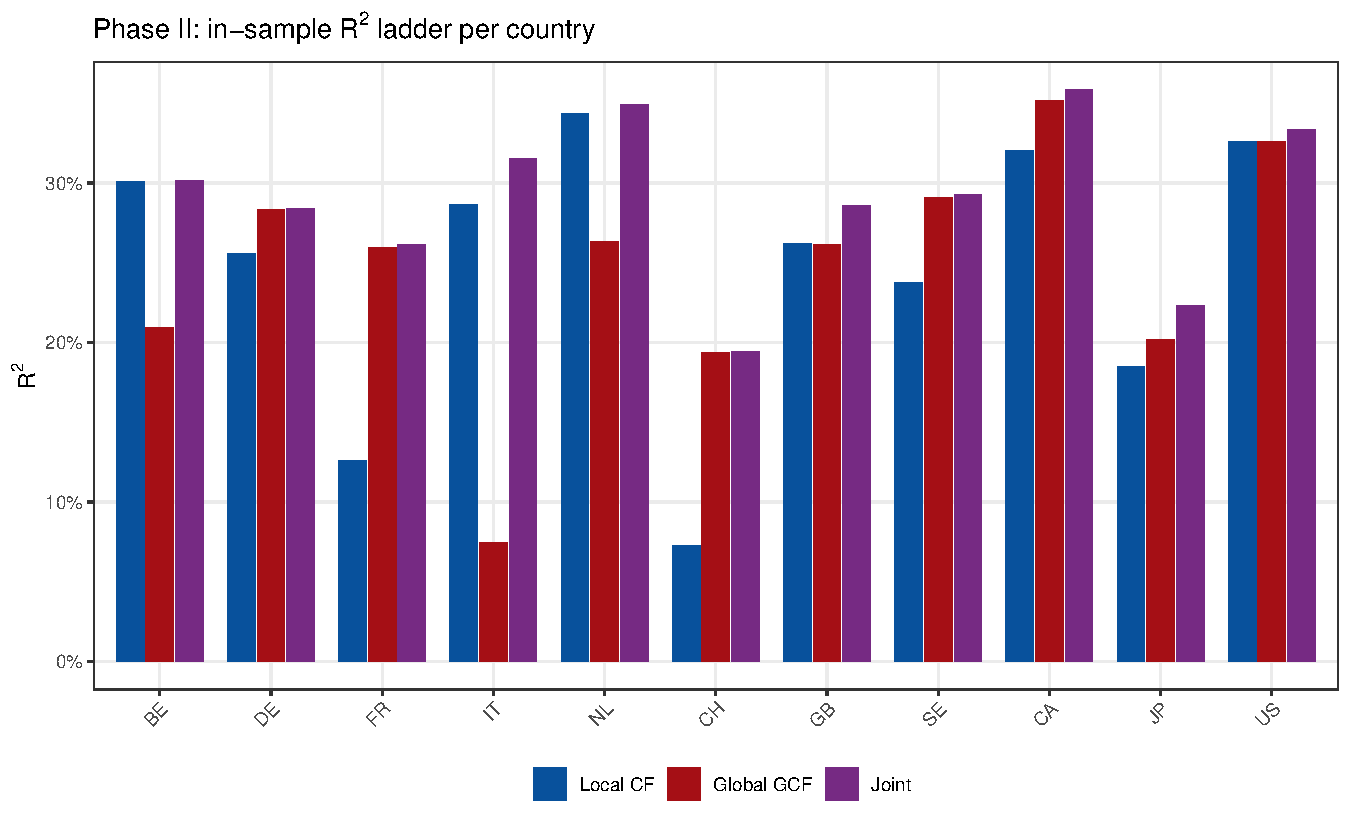
\includegraphics[width=0.85\linewidth]{figures/mr_f2_r2_ladder.pdf}
\end{frame}

\begin{frame}{Appendix: Phase III --- USD-Investor Table}
  \centering
  % mr_t3_phase3 — Phase III: US-dollar investor, GCF vs the FX-adjusted FXGCF.
% Native-LaTeX version for the deck; numbers match thesis/tables/mr_t3_phase3.tex
% (generated by main_results.R). Replaces the former PDF screenshot.
\setlength{\tabcolsep}{4pt}
\resizebox{\linewidth}{!}{%
\begin{tabular}{l c ccc ccc r}
  \toprule
  & & \multicolumn{3}{c}{$\GCF_{t}$} & \multicolumn{3}{c}{$\FXGCF_{t}$} & \\
  \cmidrule(lr){3-5}\cmidrule(lr){6-8}
  Country & $R^{2}$ ($\CF$) & $\hat{\gamma}$ & $t$ & $R^{2}$ & $\hat{\delta}$ & $t$ & $R^{2}$ & $N$ \\
  \midrule
  Belgium        & $0.032$ & $1.73$ & $(1.58)$ & $0.048$ & $1.24$ & $(1.84)$ & $0.068$ & $353$ \\
  Germany        & $0.065$ & $1.75$ & $(1.60)$ & $0.050$ & $1.25$ & $(1.85)$ & $0.071$ & $353$ \\
  France         & $0.083$ & $1.75$ & $(1.62)$ & $0.050$ & $1.24$ & $(1.88)$ & $0.070$ & $353$ \\
  Italy          & $0.109$ & $1.65$ & $(1.53)$ & $0.041$ & $1.15$ & $(1.73)$ & $0.054$ & $353$ \\
  Netherlands    & $0.011$ & $1.75$ & $(1.60)$ & $0.050$ & $1.25$ & $(1.86)$ & $0.070$ & $353$ \\
  Switzerland    & $0.146$ & $1.51$ & $(1.52)$ & $0.044$ & $1.11$ & $(1.83)$ & $0.066$ & $353$ \\
  United Kingdom & $0.114$ & $1.70$ & $(1.95)$ & $0.070$ & $1.07$ & $(1.98)$ & $0.077$ & $353$ \\
  Sweden         & $0.098$ & $2.48$ & $(1.96)$ & $0.074$ & $1.67$ & $(2.17)$ & $0.092$ & $353$ \\
  Canada         & $0.114$ & $2.12$ & $(2.85)$ & $0.126$ & $1.39$ & $(2.99)$ & $0.148$ & $353$ \\
  Japan          & $0.000$ & $0.46$ & $(0.34)$ & $0.002$ & $0.61$ & $(0.79)$ & $0.009$ & $367$ \\
  United States  & $0.326$ & $1.38$ & $(4.40)$ & $0.326$ & $0.83$ & $(4.08)$ & $0.324$ & $412$ \\
  \bottomrule
\end{tabular}}\\[0.8ex]
{\scriptsize\begin{minipage}{0.96\linewidth}
  Dependent variable: the US-dollar excess return
  $\rxbar^{\,\mathrm{USD}}_{i,t+12}$. The first column repeats the $R^{2}$ of the
  dollar return on the local factor $\CF_{i,t}$ for reference; the $\GCF$ and
  $\FXGCF$ blocks regress on the global and FX-adjusted global factors.
  Newey--West HAC $t$-statistics in parentheses. The US row carries no currency
  leg. In this sample $\Corr(\GCF_{t},\FXGCF_{t})=0.99$.
\end{minipage}}

\end{frame}

\begin{frame}{Appendix: Out-of-Sample Summary Table}
  \centering
  % mr_t4_oos — Out-of-sample summary: recursive Campbell-Thompson R2 by phase.
% Native-LaTeX version for the deck; numbers match thesis/tables/mr_t4_oos.tex
% (generated by main_results.R). Replaces the former PDF screenshot.
\resizebox{0.95\linewidth}{!}{%
\begin{tabular}{ll ccc}
  \toprule
  Phase & Specification & In-sample $R^{2}$ (mean) & $R^{2}_{\mathrm{oos}}$ (pooled) & Markets OOS$+$ \\
  \midrule
  I --- local          & $\rxbar \sim \CF$                       & $0.247$ & $-0.076$ & $2/11$  \\
  II --- global        & $\rxbar \sim \GCF$                      & $0.247$ & $0.046$  & $10/11$ \\
  III --- USD, global  & $\rxbar^{\,\mathrm{USD}} \sim \GCF$     & $0.080$ & $-0.071$ & $2/11$  \\
  III --- USD, FX-adj. & $\rxbar^{\,\mathrm{USD}} \sim \FXGCF$   & $0.095$ & $0.002$  & $9/11$  \\
  \bottomrule
\end{tabular}}\\[0.8ex]
{\scriptsize\begin{minipage}{0.92\linewidth}
  In-sample $R^{2}$ is the cross-country mean of the single-factor fits. The
  out-of-sample $R^{2}_{\mathrm{oos}}$ is the pooled
  \citet{campbellthompson2008} statistic of the fully recursive factor forecast
  relative to the recursive prevailing mean; positive means the factor beats the
  real-time historical average. Both factor construction and forecasting
  regression respect time-$t$ information (doubly out of sample). The two
  $R^{2}$ columns use different benchmarks and are not comparable in level.
\end{minipage}}

\end{frame}

\begin{frame}{Appendix: Strategy Performance}
  \centering
  % strat_t1_performance — OOS performance of the GCF bond-timing strategy.
% Native-LaTeX version for the deck, numbers match thesis/tables/strat_t1_performance.tex
% (generated by strategy.R). Replaces the former PDF screenshot.
\resizebox{0.95\linewidth}{!}{%
\begin{tabular}{l c c c c c}
  \toprule
  Strategy & Mean (\%) & Vol (\%) & Sharpe & CER, $\gamma=5$ (\%) & CER, $\gamma=10$ (\%) \\
  \midrule
  $\GCF$-timed          & $3.02$ & $7.89$ & $0.38$ & $1.46$ & $-0.10$ \\
  Recursive-mean timing & $2.39$ & $7.00$ & $0.34$ & $1.16$ & $-0.07$ \\
  Buy-and-hold          & $2.17$ & $6.98$ & $0.31$ & $0.95$ & $-0.27$ \\
  \bottomrule
\end{tabular}}\\[0.8ex]
{\scriptsize\begin{minipage}{0.92\linewidth}
  Real-time performance of timing a 10Y GDP-weighted global bond portfolio with
  the global cycle factor over 2005--2024 ($n=221$ months, portfolio
  $R^{2}_{\mathrm{oos}}=0.12$). Exposure follows the mean--variance rule
  $w_{t}\propto\widehat{\E}_{t}[\rx_{t+12}]/\widehat{\sigma}^{2}_{t}$ with the
  recursive $\GCF^{\mathrm{oos}}$ forecast. CER is the annual certainty equivalent for
  risk aversion $\gamma$. Local-currency (hedged) 12-month excess
  returns.
\end{minipage}}

\end{frame}

\begin{frame}{Appendix: Robustness --- Subsample Stability}
  \centering
  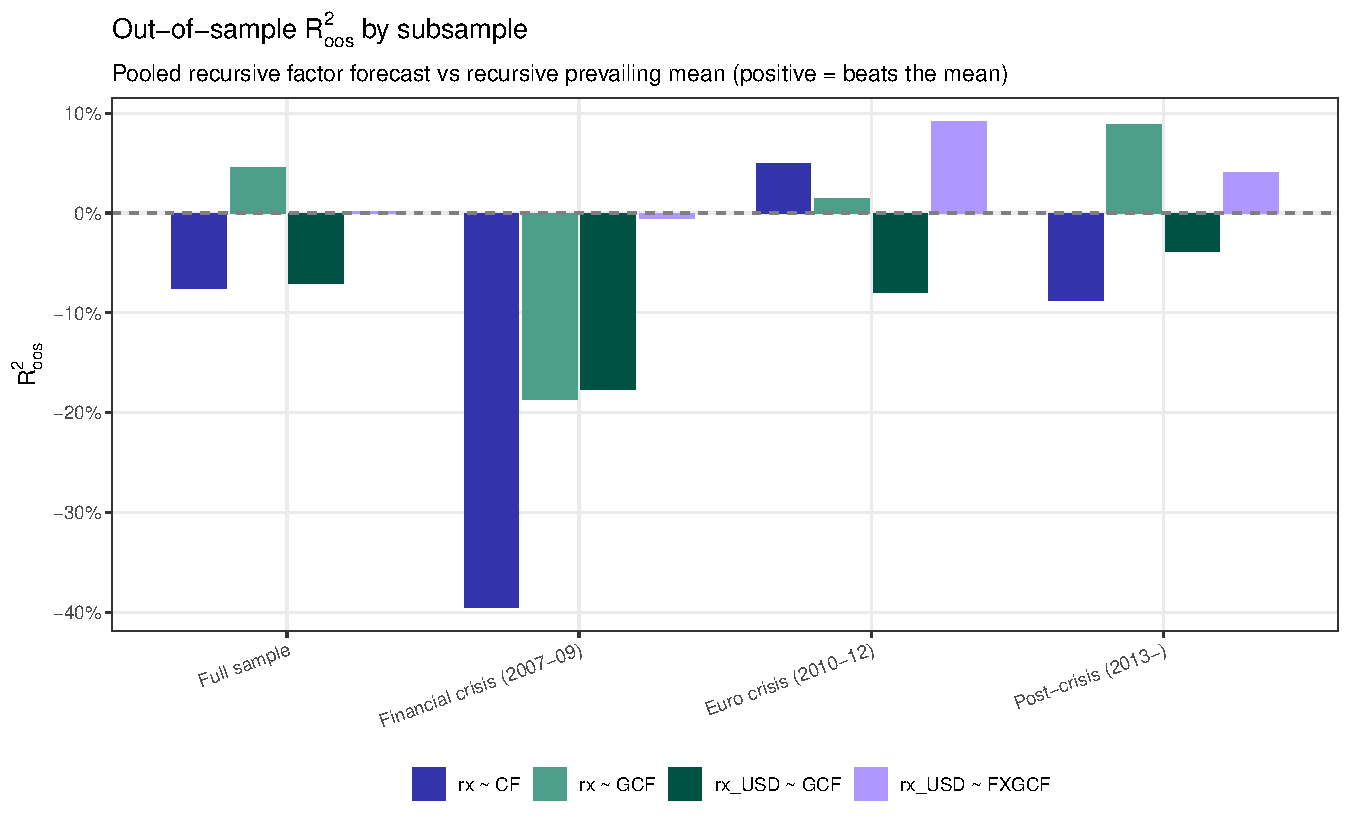
\includegraphics[height=0.40\textheight]{figures/rob_f1_oos_sub.pdf}\\[0.5ex]
  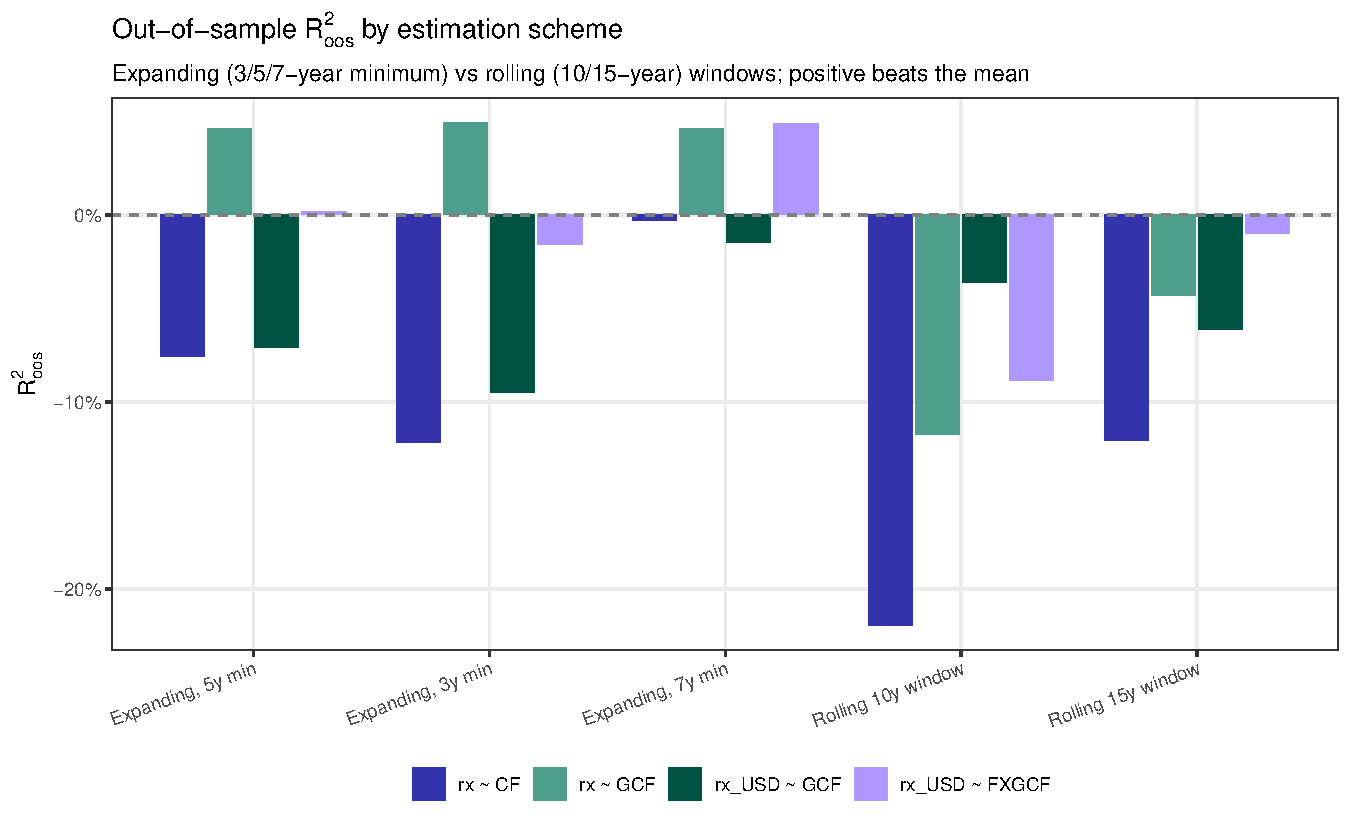
\includegraphics[height=0.40\textheight]{figures/rob_f2_oos_scheme.pdf}
\end{frame}

\begin{frame}{Appendix: G10 Countries}
  \begin{columns}[T]
    \begin{column}{0.5\textwidth}
      \begin{itemize}
        \item Belgium
        \item Canada
        \item France
        \item Germany
        \item Italy
        \item Japan
      \end{itemize}
    \end{column}
    \begin{column}{0.5\textwidth}
      \begin{itemize}
        \item Netherlands
        \item Sweden
        \item Switzerland
        \item United Kingdom
        \item United States
      \end{itemize}
    \end{column}
  \end{columns}
\end{frame}

\end{document}
